\section{Validación}
\subsection{Métodos}
La validación realizada para este proyecto consistió en una encuesta que debe contestar dos expertos y una empresa. Los dos expertos son Mario Murcia y María Angélica Parra, los dos son expertos en temas relacionados con los ecosistemas y el agua. Por otro lado, la empresa que ha validado la herramienta desarrollada es Corona, en especial la división independiente de Corona, Empresa Colombiana de Cementes (Alion). Alion es una división independiente de Corona cuyo origen es una alianza con Cementos Molins de España. Esta división comenzó operaciones en el 2019-2 y se especializa en la extracción de caliza en Río Claro. Alion es el proveedor principal de insumos de otras divisiones de Corona como, por ejemplo, Insumos Industrias y Energía. 
Para la validación de la aplicación web, proveniente del modelo producto de la estrategia, se realizó un formulario en Google Forms. Este formulario busca evaluar los atributos de calidad de la aplicación web, la calidad de preguntas con respecto al contexto del agua como capital natural y otros atributos que se deben evaluar de la aplicación. En la tabla \ref{tab:formulari-validacion} en el Apéndice A podrá ver las preguntas que se realizaron en el formulario. Por cada atributo evaluado se incluyó una sección abierta para que el evaluador pudiera incluir comentarios adicionales.

Las preguntas relacionadas al contexto, practicidad, visualizaciones finales y utilidad están evaluando de manera indirecta a la estrategia. Esto se debe a que están evaluando la calidad del modelo, la facilidad de usar la herramienta y por lo tanto la estrategia, la claridad de las visualizaciones finales, i.e., los resultados de la estrategia y la utilidad de la herramienta, es decir, si los resultados han ayudado a la empresa a entender su situación actual.

\subsection{Validación de resultados}
En esta sección se discutirá los resultados de las validaciones hechas por los expertos. Los cuatro atributos de calidad evaluados de la aplicación web fueron la funcionalidad, la confiabilidad, la usabilidad y el rendimiento. En la segunda pregunta relacionada a la funcionalidad de la herramienta, “¿Encontró alguna función que no estuviera disponible y que considere esencial?”, hubo un comentario que mencionaba que hacía falta el servicio ecosistémico ‘Cultural del Agua’. Este error pudo haber sido causado por una falta de atención en el momento de copiar la información entregada por el experto a la aplicación.  En esta sección también se hizo el comentario de una mayor explicación en la sección de indicadores puesto que la búsqueda en los documentos de estos no es inmediata y se puede caer en imprecisiones. En la siguiente imagen se podrá ver las respuestas a la primera pregunta de la validación. Como se puede ver, tanto a los expertos como a la empresa, estaban todas las necesidades para evaluar las dependencias e impactos de la empresa sobre el agua.

\begin{figure}[H]
        \centering
        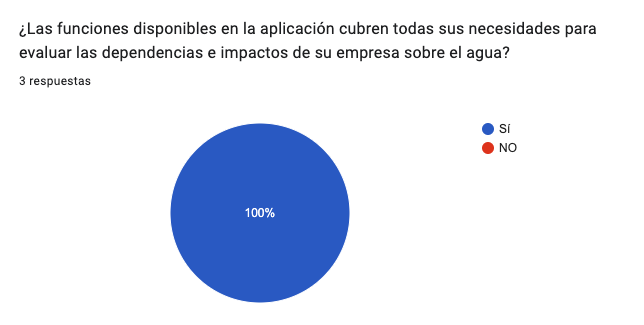
\includegraphics[scale=0.45]{images/6-validacion/1-funcionalidad.png}
        \caption{Respuestas de la primera pregunta relacionada a la funcionalidad de la aplicación web}
 \end{figure}

Con respecto a la confiabilidad, el único comentario que se obtuvo fue que la aplicación permitía continuar a la siguiente pregunta sin haber respondido la pregunta. Este comportamiento está basado en el comportamiento de la herramienta de IMPULS Industry 4.0 Readiness Online Self-Check for Business, la cual le permite a las empresas hacer todo el diagnóstico sin haber respondido todas las preguntas. Por otro lado, en ninguna de las validaciones hechas por los usuarios hubo pérdida de datos o información incorrecta al usar la aplicación.

\begin{figure}[H]
        \centering
        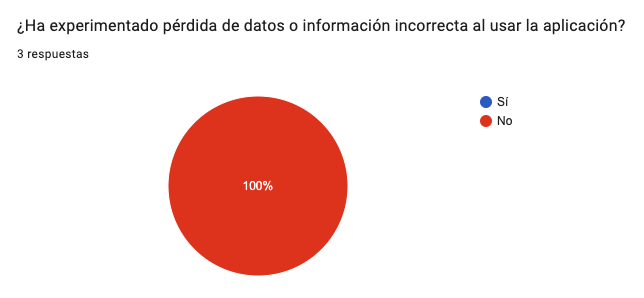
\includegraphics[scale=0.45]{images/6-validacion/2-confiabilidad.png}
        \caption{Porcentaje de pérdida de datos o información según evaluadores}
\end{figure}

La ‘Usabilidad’ de la herramienta tuvo un gran resultado pues los evaluadores se demoraron menos de 30 minutos en familiarizarse con el uso de la aplicación y el 66\% de los evaluadores consideraron la interfaz intuitiva y fácil de usar. Sin embargo, los comentarios si mencionaban como era importante advertir a la empresa que utilice la herramienta la necesidad de tener la información lista o saber dónde está para así agilizar el proceso.  Adicionalmente, se recomienda disminuir el número de preguntas para hacer el tiempo de respuesta mucho menor.

\begin{figure}[H]
        \centering
        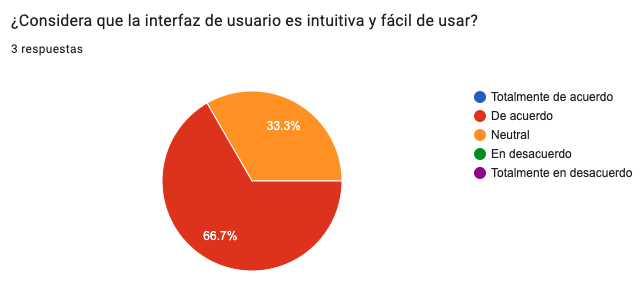
\includegraphics[scale=0.45]{images/6-validacion/3-usabilidad.png}
        \caption{Porcentaje de evaluadores que consideran la interfaz intuitiva y fácil de usar}
\end{figure}

\begin{figure}[H]
        \centering
        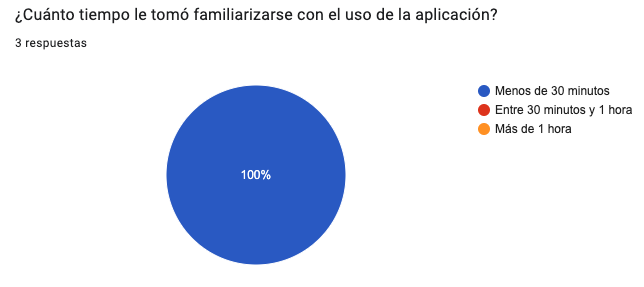
\includegraphics[scale=0.45]{images/6-validacion/4-usabilidad.png}
        \caption{Tiempo para familiarizarse con la aplicación según evaluadores}
\end{figure}
    
El rendimiento de la aplicación tuvo, en términos generales, una respuesta positiva ya que la velocidad de carga fue, por lo menos, satisfactoria. Pero, si hubo un comentario en el cual se mencionaba que había preguntas que se demoraban en salir lo que posiblemente dejaba preguntas sin responder. 

\begin{figure}[H]
        \centering
        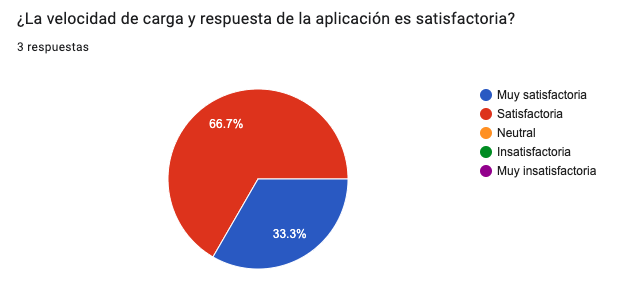
\includegraphics[scale=0.45]{images/6-validacion/5-rendimiento.png}
        \caption{Satisfacción de los evaluadores con respecto a la velocidad de carga y respuesta de la aplicación}
\end{figure}
 
\begin{figure}[H]
        \centering
        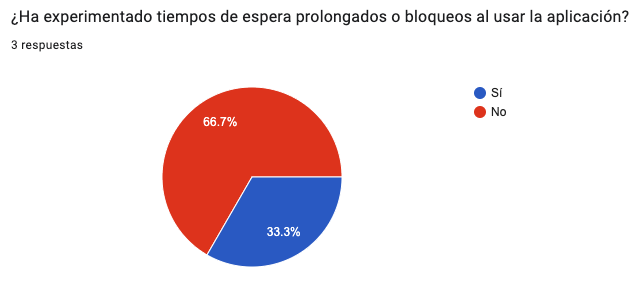
\includegraphics[scale=0.45]{images/6-validacion/6-rendimiento.png}
        \caption{Respuestas con respecto al rendimiento de la aplicación}
\end{figure}
 
  
Con respecto a la consideración del ‘Contexto’, la aplicación puede mejorar en la información mínima para que la empresa pueda entender su nivel de madurez. Adicionalmente, se puede mejorar la redacción de algunas de las preguntas hechas en el cuestionario. Finalmente, en la sección de comentarios se advierte de que la herramienta es útil para empresas reguladas, pero para empresas no reguladas podría ser un reto responder la mayoría de las preguntas. 

\begin{figure}[H]
        \centering
        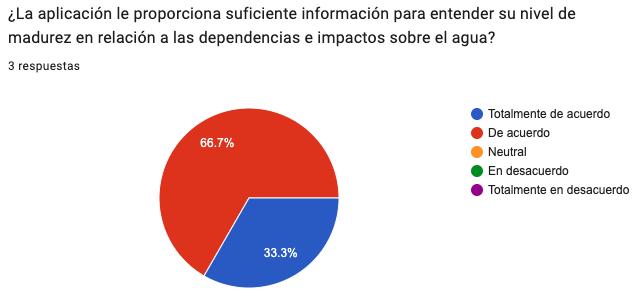
\includegraphics[scale=0.45]{images/6-validacion/7-contexto.png}
        \caption{Percepción de los evaluadores con respecto a la cantidad de información proporcionada por la aplicación para entender el nivel de madurez}
\end{figure}

\begin{figure}[H]
        \centering
        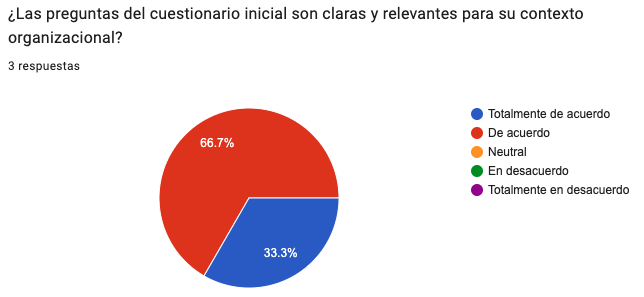
\includegraphics[scale=0.45]{images/6-validacion/8-contexto.png}
        \caption{Claridad y relevancia de las preguntas del cuestionario según los evaluadores}
\end{figure}


Para las visualizaciones finales de la aplicación donde se muestra el nivel de madurez y las relaciones el comentario principal fue la necesidad de simplificar las gráficas. Ya sea través de explicaciones más claras de cómo utilizar las gráficas o cambiar el tipo de gráficas que se utilizan. Esta inconformidad se puede ver en las gráficas presentadas a continuación. En especial, en la gráfica que muestra los resultados de la pregunta que evalúa la utilidad para los análisis de las gráficas. 


\begin{figure}[H]
        \centering
        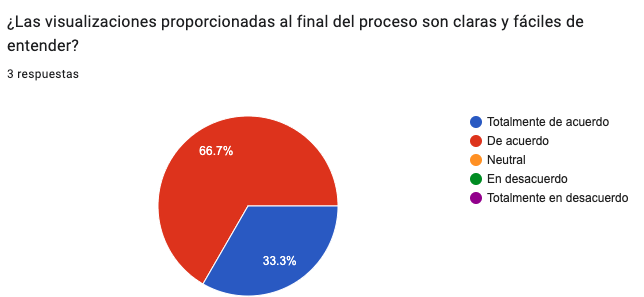
\includegraphics[scale=0.45]{images/6-validacion/9-vf.png}
        \caption{Claridad y facilidad de entender de las visualizaciones según los evaluadores}
\end{figure}
    
\begin{figure}[H]
        \centering
        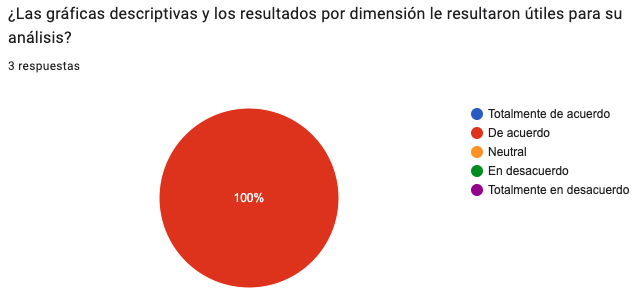
\includegraphics[scale=0.45]{images/6-validacion/10-vf.png}
        \caption{Gráficas descriptivas para entender los resultados relacionados a las dimensiones evaluadas}
\end{figure}

 

La utilidad de la aplicación tuvo grandes resultados ya que la aplicación le ha ayudado a identificar nuevas áreas de mejora en la gestión del agua al tiempo que cumple con los objetivos establecidos.  A través de la aplicación, según los evaluadores, se pudo determinar el nivel de madurez, la mejor dimensión y exponer características descriptivas de los indicadores.

\begin{figure}[H]
        \centering
        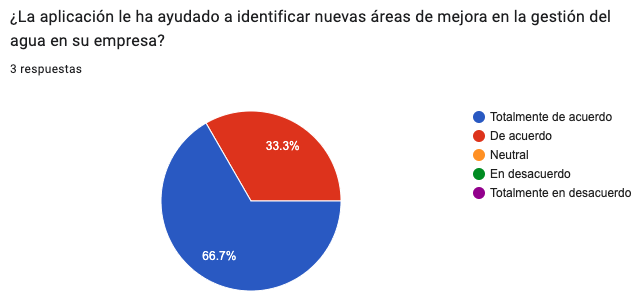
\includegraphics[scale=0.45]{images/6-validacion/11-utilidad.png}
        \caption{Utilidad para encontrar nuevas áreas de mejora}
\end{figure}

\begin{figure}[H]
        \centering
        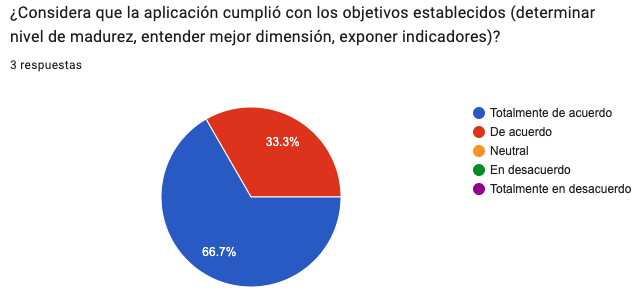
\includegraphics[scale=0.45]{images/6-validacion/12-utilidad.png}
        \caption{Percepción de los evaluadores acerca del cumplimiento de los objetivos}
\end{figure}

\hfill

Además de los resultados del formulario, la validación también se hizo de manera virtual con el represéntate de Corona y Alion, como mencionado anteriormente. Durante esta validación el represéntate tuvo algunas preguntas con respecto a la herramienta. Primero, el representante preguntó si existía la posibilidad de poder ver los resultados de otras empresas para poder compararlos con los de su empresa. Esta funcionalidad, sin embargo, todavía no está implementada. Esto se debe a que esta herramienta sigue siendo un prototipo y su objetivo principal era determinar el nivel de madurez de su propia empresa. Sin embargo, esta funcionalidad se podría implementar dependiendo de cuantas empresas utilicen el prototipo puesto que la funcionalidad se nutriría de la misma información proporcionada por las empresas. El representante de Corona y Alion también estaba interesado en ver sus respuestas específicas para cada una de las variables del modelo. Esta funcionalidad sería una extensión de la aplicación web ya que, para obtener un mejor resultado, hacer un tablero de control en herramientas como Power BI o Tableau presentaría un mejor informe a la empresa. Finalmente, el representante de Corona y Alion hizo comentarios con respecto a la facilidad de uso de la aplicación con respecto a ciertos esfuerzos adicionales que se debían hacer. Por ejemplo, el representante no se escuchaba a gusto con el hecho de tener que guardar manualmente las respuestas. La razón detrás de dicho protocolo es por la capacidad de los servicios utilizados para este prototipo. Debido a que el servidor donde corría la aplicación web, Render, y la base de datos donde se almacenaba los datos, Mongo DB, estaban con planes gratuitos, las limitaciones tecnológicas no permitan el guardado automático constantemente. Para evitar errores o comportamientos indeseados durante la utilización de la aplicación, se tomó la decisión de hacer un guardado manual o un guardado cuando se acabara todo un paso por completo.
